\documentclass[a4paper,14pt]{scrartcl} 
\usepackage[T2A]{fontenc}
\usepackage[utf8]{inputenc}
\usepackage[english,russian]{babel}
\selectlanguage{Russian}
\usepackage{afterpage}
\usepackage{amsmath}
\usepackage{graphicx}
\usepackage{listings}
\usepackage{wrapfig}
\usepackage{setspace}
\doublespacing
\usepackage{pdfpages}
\usepackage{courier}
\lstset{basicstyle=\footnotesize\ttfamily,breaklines=true}
\usepackage{enumitem}
\addto\captionsenglish{\renewcommand\contentsname{Оглавление}}
\addto\captionsenglish{\renewcommand\figurename{Рис.}}


\begin{document}


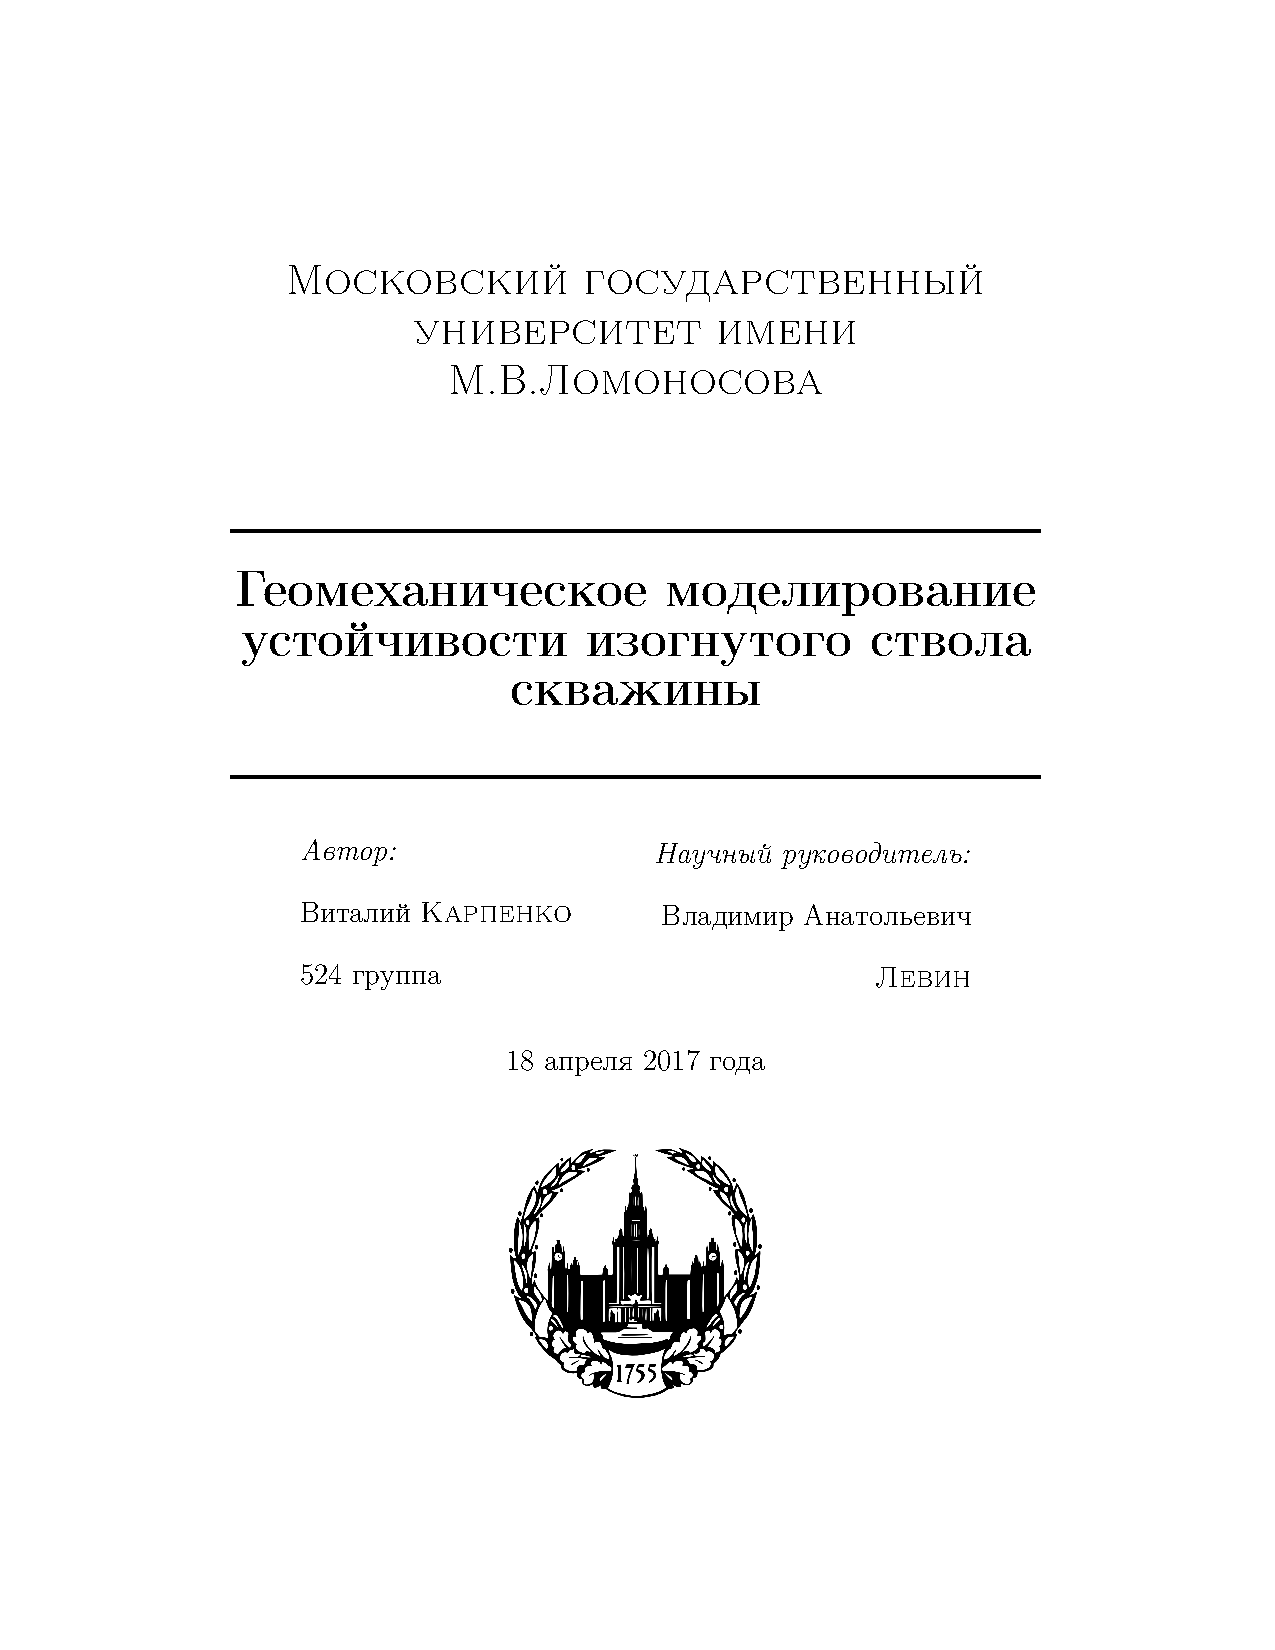
\includepdf[pages=1]{title.pdf}


\tableofcontents


\newpage
\section{Введение}
\subsection{О задаче}
Определение технологических параметров, при которых ствол скважины будет сохранять стабильное состояние – одна из важнейших задач геомеханики. Одним из параметров, которые могут относительно легко контроллироваться человеком и при этом оказывают значительное влияние на устойчивость (в каком смысле в данной работе употребляется этот термин будет пояснено далее), является плотность бурового раствора, который заливается в скважину во время бурения. Столб жидкости создаёт дополнительное давление в стволе, служащее "опорой", не позволяющей геометрии скважины уйти в область пластических деформаций под действием давления окружающих слоёв горных пород. 

\subsection{О работе}
В работе описывается разработка программы на языке Python, позволяющей по каротажным данным (т.е. информации о форме скважины, окружающих породах и т.д., полученной с помощью спуска-подъёма в скважине геофизического зонда) автоматически строить соответствующую им модель в препроцессоре CAE Fidesys и производить расчёт для определения оптимальной плотности бурового раствора - он должен быть достаточно плотным, чтобы удерживать ствол скважины от слишком сильных деформаций, но при этом не быть слишком плотным, чтобы не мешать процессу бурения.


\newpage
\section{Механическая постановка задачи}
\begin{itemize}
    \item Рассматривается изогнутая скважина круглого сечения (радиус может не быть константным).
    \item Деформации считаются малыми.
    \item Исследуется только область отстоящая от стенок скважины на расстояние $10r$, где $r$ - радиус скважины. Расположенные дальше горные породы нас не интересуют, т.к. к скважине прикладывается только давление столба жидкости, интеграл от которого по любому сечению, перпендикулярному направлению ствола, равен $0$ в силу симметрии. Следовательно, по принципу Сен-Венана, с удалением от концентратора напряжений (т.е. скважины) дополнительные напряжения, вызванные наличием скважины, будут затухать и на расстоянии на порядок превышающем характерный размер концентратора мы можем считать их пренебрежимо малыми.
    \item Материал упруго-пластический Друкера-Прагера.
    \item Свойства материала изменяются по оси OZ в соответствии с каротажными данными.
    \item Изнутри стенки скважины действует забойное давление.
\end{itemize}
\afterpage{%
\begin{wrapfigure}{R}{1\textwidth}
    \centering
    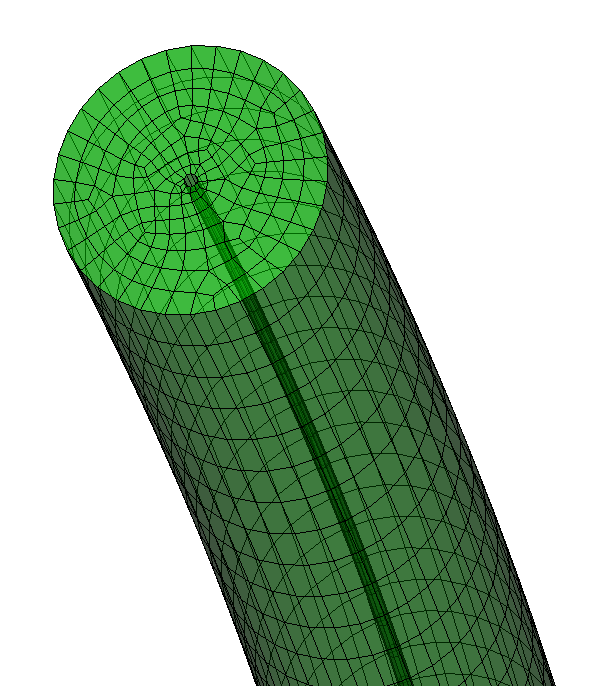
\includegraphics[width=1\textwidth]{images/well.png}
    \caption{\label{fig:well}Устье скважины.}
\end{wrapfigure}
\clearpage
}


\newpage
\section{Математическая постановка задачи}
\begin{enumerate}
    \item Уравнения равновесия:
        $$
            \sigma_{ij,j} + \rho F_i = 0;
        $$
    \item Закон Гука для упругопластической среды:
        $$
            \dot{\sigma_{ij}} = \lambda(\dot{\theta} - \dot{\theta}^p) + 2 \mu (\dot{\varepsilon_{ij}} - \dot{\varepsilon_{ij}}^p);
        $$
    \item Выражение компонент тензора деформаций через компоненты вектора перемещения:
        $$
            \dot{\varepsilon_{ij}} = \dfrac{1}{2}(u_{i,j} + u_{j,i});
        $$
    \item Приращение полных деформаций представляется в виде суммы пластической и упругой составляющих:
        $$
            \dot{\varepsilon_{ij}} = \dot{\varepsilon_{ij}}^e + \dot{\varepsilon_{ij}}^p;
        $$
    \item Упругое состояние среды в пространстве напряжений ограничено поверхностью предельного состояния. f – уравнение предельной поверхности, g – пластический потенциал, $d\lambda$ - пластический множитель, определяемый в ходе процесса деформации.
        $$
            f(\sigma_{ij}, \dot{\varepsilon}^p_{ij}) = 0;
        $$
        $$
            g(\sigma_{ij}, \dot{\varepsilon}^p_{ij}) = 0;
        $$
        $$
            d\varepsilon^p_{ij} = d \lambda \dfrac{\partial g}{\partial \sigma_{ij}};
        $$
        Предельная поверхность записывается в следующем виде (a и Y – параметры, которые можно получить, используя данные .las файла, содержащего каротажные данные (а именно коэффициент внутреннего трения и когезию). Здесь $\tau = (s_{ij} s_{ij} / 2)^{\tfrac{1}{2}}$ - интенсивность касательных напряжений:
        $$
            f(\sigma, \tau) = \tau - \alpha \sigma - Y;
        $$
        Пластический потенциал записывается в следующем виде ($\lambda$ - коэффициент дилатансии):
        $$
            g(\sigma, \tau) = \tau - \Lambda \sigma;
        $$
\end{enumerate}


\newpage
\section{Автоматическая генерация скрипта для препроцессора CAE Fidesys}
Так как скважина может иметь нетривиальную геометрию, а горные породы вокруг неё могут иметь сложную слоистую структуру, требуется способ автоматически генерировать скрипт для препроцессора, отражающий параметры задачи. Мной была разработана программа на языке Python, на вход получающая .las файл, содержащий разнообразные данные, полученные с помощью опускания геофизического зонда в ствол скважины. Файл считывается программой, анализируется, с учётом известного синтаксиса .las формата, вся информация из него считывается во внутренние структуры данных, преобразовывается для удобства работы. На этой основе формируется скрипт для препроцессора с командами, задающими геометрию шахты, свойства материалов, краевые условия и т.д.

\vspace{10mm}
\textbf{Пример фрагмента файла с каротажными данными:} 
\begin{lstlisting}[frame=single]
~Metadata
...
~Curve information
Depth
TVD
Pw
zen
azi
...
~A LOG DATA SECTION
1020.2000 1020.2000 10.0000 0.0000 219.0000 ...
1020.4000 1020.4000 10.0020 0.0000 219.0000 ...
\end{lstlisting}

\newpage
\textbf{Пример фрагмента сгенерированного скрипта для препроцессора:} 
\begin{lstlisting}[frame=single]
reset
set node constraint on
open well_geometry.fds
curve 13 interval 10
curve 13 scheme equal
mesh curve 13
surface 12 size 0.8
mesh surface 12
create material "grunt" property_group "HOOK_DRUCKER_PRAGER" 
block 1 add volume 1
block 1 element type hex20
block 1 material 'grunt'
create table 101 file Edyn.csv
modify table 101 dependency z
modify material 1 set property 'MODULUS' table 101
\end{lstlisting}

\subsection{Дополнительная информация о формате .las}
Аббревиатура LAS является сокращением от Log ASCII Standard (ASCII – American Standard Code for Information Interchange).
Формат Las разрабатывался с целью быть хорошо читаемым для рядовых пользователей, но в то же время не создавать сложностей программистам для написания программ, записывающих или изменяющих файлы данного формата по известным правилам. Во-первых, файлы формата Las – это всегда текстовые файлы, которые можно легко открыть и просмотреть с помощью любого текстового редактора.  Для удобства распознавания файла LAS среди всех остальных файлов, он должен иметь соответствующее расширение - “.LAS”. Las-файл состоит из нескольких разделов (секций). Порядок их размещения никак не регламентируется, за исключением того, что секция данных должна быть последней секцией в файле. Как правило, первым разделом записывается раздел “VERSION”, несущий в себе информацию об используемой версии формата. В секции “WELL INFORMATION” заключена информация о скважине, ее имени, положении и т.п. Раздел “CURVE INFORMATION” перечисляет имена каротажных кривых, записанных в данном файле. Секции “PARAMETER” и “OTHER” не являются обязательными и не всегда присутствуют в файле. Первая из них описывает различные параметры, относящиеся к скважине (такие, как сопротивление и вязкость бурового раствора). Вторая применяется для записи комментариев. Последней секцией файла обязательно должна быть секция “ASCII LOG DATA”. Здесь записываются колонки данных, отделенных друг от друга пробелами.

\newpage
\section{Рассмотрение решения конкретной задачи.}
\subsection{Форма скважины, построенной по данному заказчиком .las файлу}
\vspace{100px}
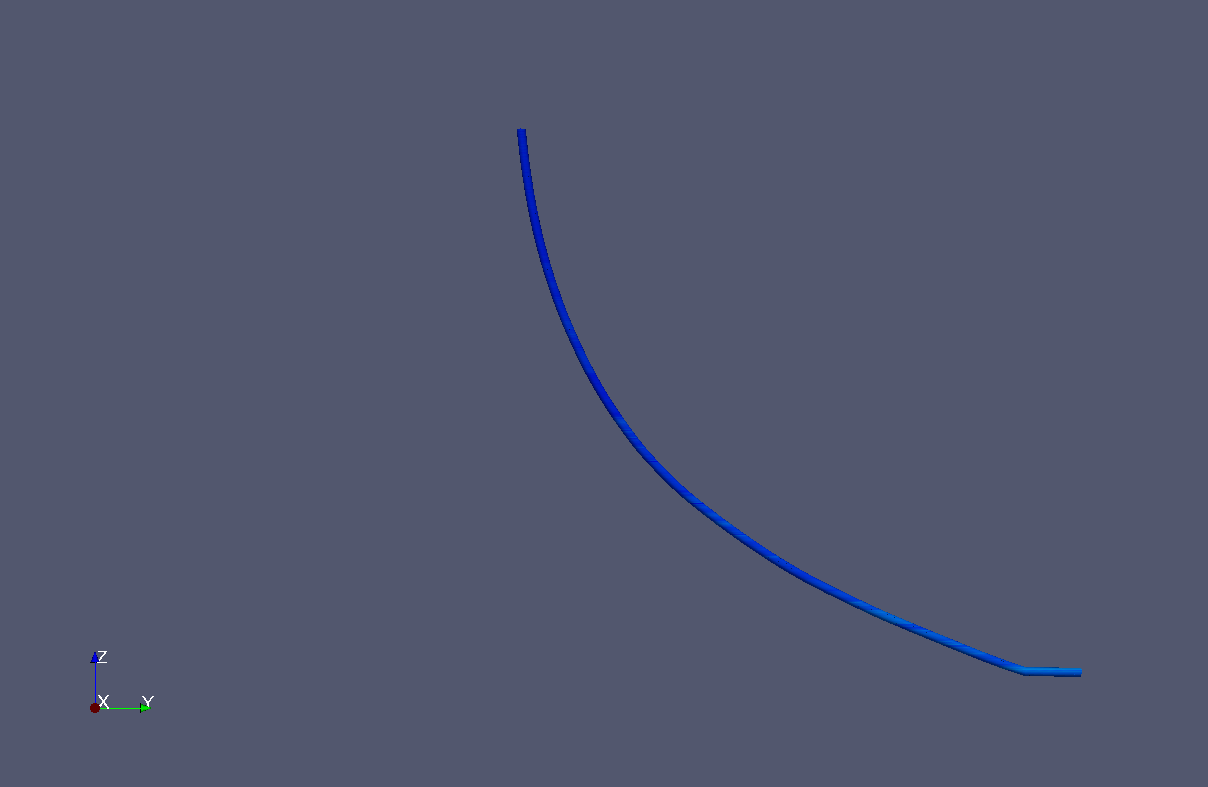
\includegraphics[width=1\textwidth]{images/form.png}
\afterpage{%
\subsection{Слоистая структура окружающих горных пород.}
При более близком рассмотрении любого из участков скважины хорошо заметно, что породы вокруг скважины, как и ожидалось, имеют ярко выраженную слоистую структуру. \\

\vspace{100px}
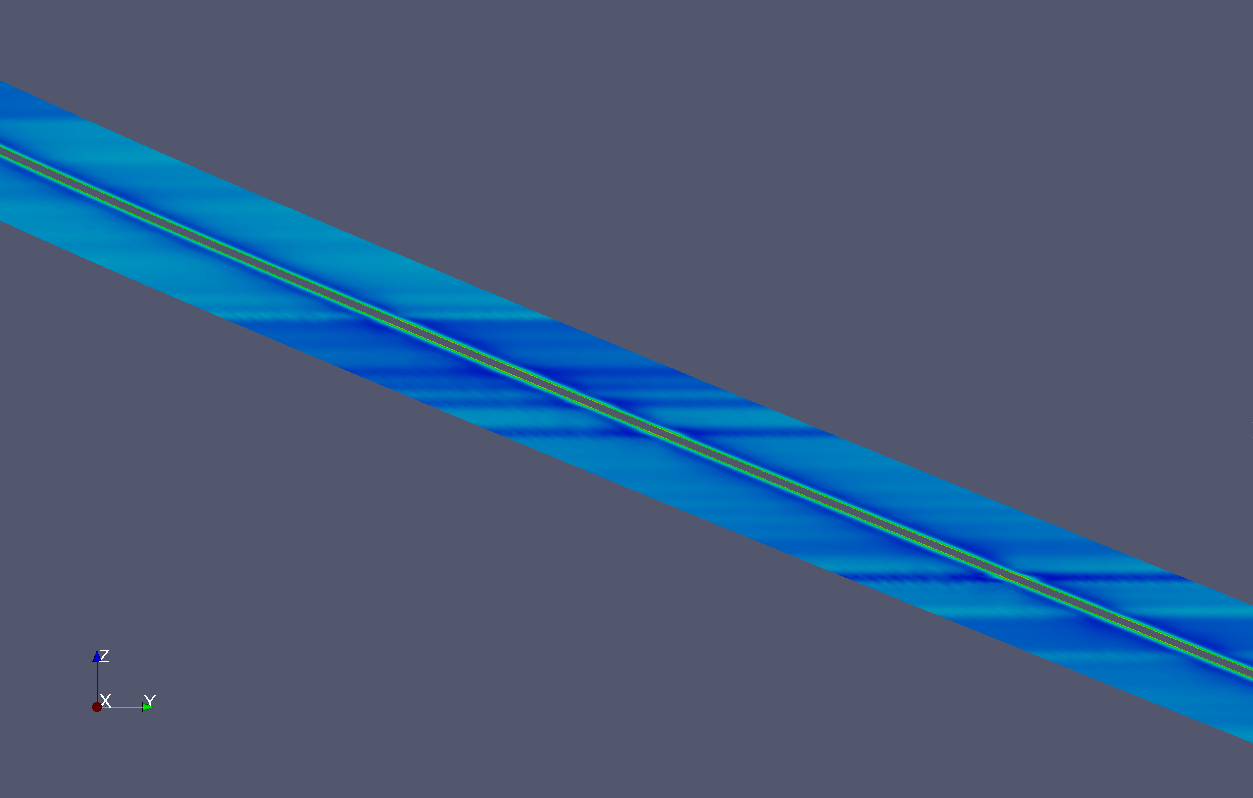
\includegraphics[width=1\textwidth]{images/layers.png}
\clearpage
}

\newpage
\subsection{Два варианта расчёта.}
\vspace{20px}
\noindent
\begin{minipage}{.5\textwidth}
    1) \textbf{Без забойного давления.}

    Проверяется НДС скважины исключительно под действием веса окружающих горных пород.
\end{minipage}
\hspace{20px}
\begin{minipage}{.5\textwidth}
    2) \textbf{С забойным давлением.}

    Расчёт проводится при учёте забойного давления - т.е. давления столба бурового раствора внутри шахты.
\end{minipage}

\vspace{30px}
Как уже говорилось выше, основной вопрос, интересующий нас при решении данной задачи - достаточно ли плотности используемого бурового раствора для создания такого забойного давления, что деформации стенок скважины не будут уходить в пластическую область - иными словами, обратимы ли эти деформации.
\subsubsection{С проектировочным забойным давлением.}
Сначала я провёл расчёт, использующий значения забойного давления из предоставленного заказчиком .las файла.\newline
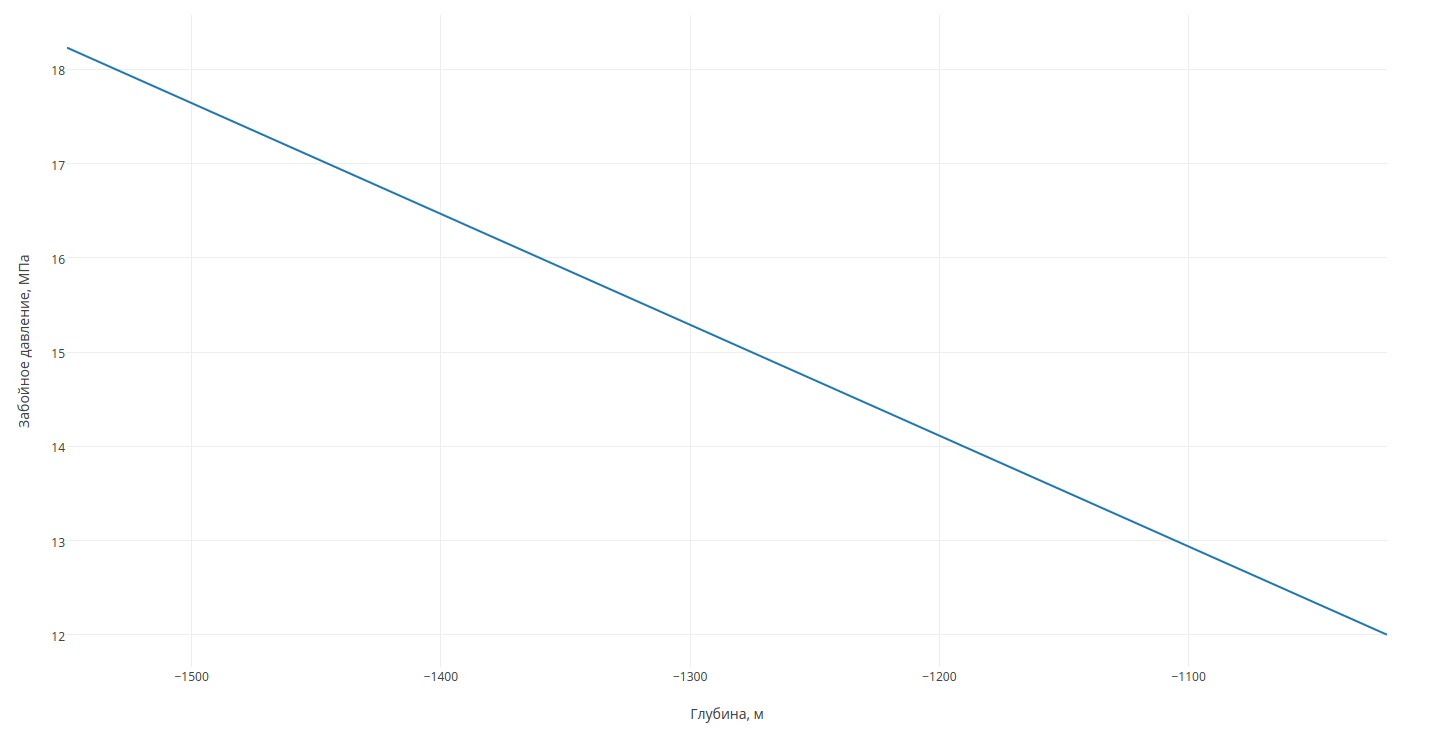
\includegraphics[width=1\textwidth]{images/pressure.png}
Результат оказался точно такой, как и ожидался - пластические деформации полностью отсутствуют полностью.\newline
\subsubsection{Без забойного давления.}
Следующий расчёт проводился, чтобы удостовериться, что не "поддерживаемая" буровым раствором скважины действительно начинает пластически деформироваться. Забойное давление из данных было полностью заменено нулевым.\newline
При отсутствии "сопротивления" в виде гидростатического напряжения бурового раствора напряжения увеличиваются несколько раз и деформации становятся пластическими.\newline

\vspace{30px}
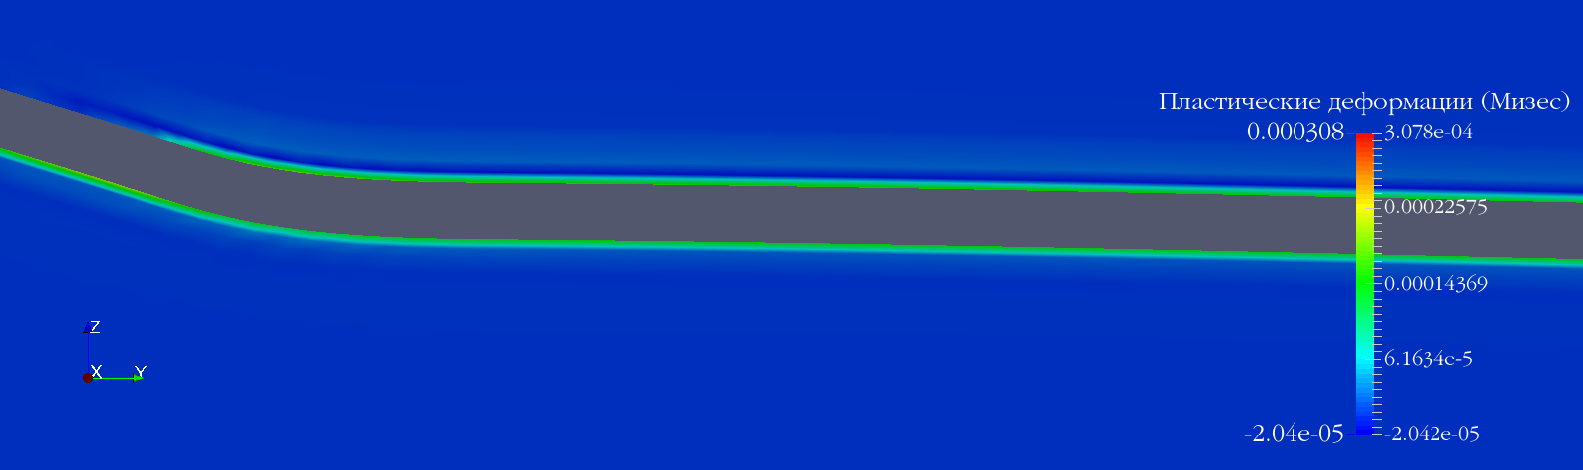
\includegraphics[width=1\textwidth]{images/plasticity.png}

\newpage
\section{Заключение.}
Был разработан алгоритм и его программная реализация на языке Python для автоматического построения МКЭ-модели в CAE Fidesys на основе данных каверномера и каротажа. При проверки программы на реальной задаче были полученные соответствующие ожиданиям результаты.
\end{document}
